\subsection{Библиотека для мобильных устройств (Вишневский Глеб)}

Основной задачей являлось создание библиотеки для обработки жестов, с помощью которой можно обучать модель и распознавать движения. Все наработки находились в Jupyter файлах, поэтому было необходимо перенести все в Python файлы, объединить и привести код в порядок. \newline

Так как наше мобильное приложение сделано с помощью JavaScript, а все основные алгоритмы – с помощью Python, то было принято решение сделать следующее: разработать библиотеку с помощью JavaScript, которая предоставляет интерфейс для обучения и предсказания движения, а внутри эта библиотека общается с Python сервером с помощью протокола http, на котором уже происходят все вычисления.

\subsubsection{JavaScript Library}
У JavaScript библиотеки определены следующие классы:
\begin{itemize}
  \item GestureData. Данный класс характеризует данные, полученные с устройства.
  \item Gesture. Данный класс характеризует распознанный жест.
\end{itemize}
В класссе Gesture содержится информация о жесте:
\begin{itemize}
  \item name -- класс, к которому он принадлежит (круг, квадрат, встряска и т.д.)
  \item 2dProjection -- 2-мерная проекция движения в плоскости
  \item 3dProjection -- 3-мерное движение в пространстве
  \item gestureData -- данные с акселерометра и гироскопа
  \item image -- ссылка на картинку, на которой изображено 2-мерное движение
\end{itemize}

У JavaScript библиотеки определены следующие методы:
\begin{itemize}
  \item train(name: String, gesture: GestureData): Promise<null> {} 
  \item predict(gesture: GestureData): Promise<Gesture> {}
\end{itemize}
Эти методы сериализуют переданные аргументы в JSON формат и отправляют их на Python сервер.


\subsubsection{Python Server}
Основная обработка данных происходит на серверной части. За основу было решено взять фреймворк Flask, который был обернут в класс Server, таким образом у Server определены следующие методы:
\begin{itemize}
  \item run(port). Запускает http сервер на определенном порту.
  \item add\_endpoint(endpoint, handler, methods). Добавляет слушателя по адресу endpoint, handler -- функция-коллбек, которая вызвается при получении нового запроса, methods -- HTTP-методы, с помощью которых возможно вызвать слушатель.
\end{itemize}

Вне зависимости от того, к какому обработчику приходит запрос, сервер всегда обрабатывает GestureData:
\begin{itemize}
  \item в первую очередь данные акселерометра фильтруются и сглаживаются, для этого был реализован метод GestrureData::normalize и GestureData::filter, \newline
  \begin{figure}[H]
    \begin{center}
        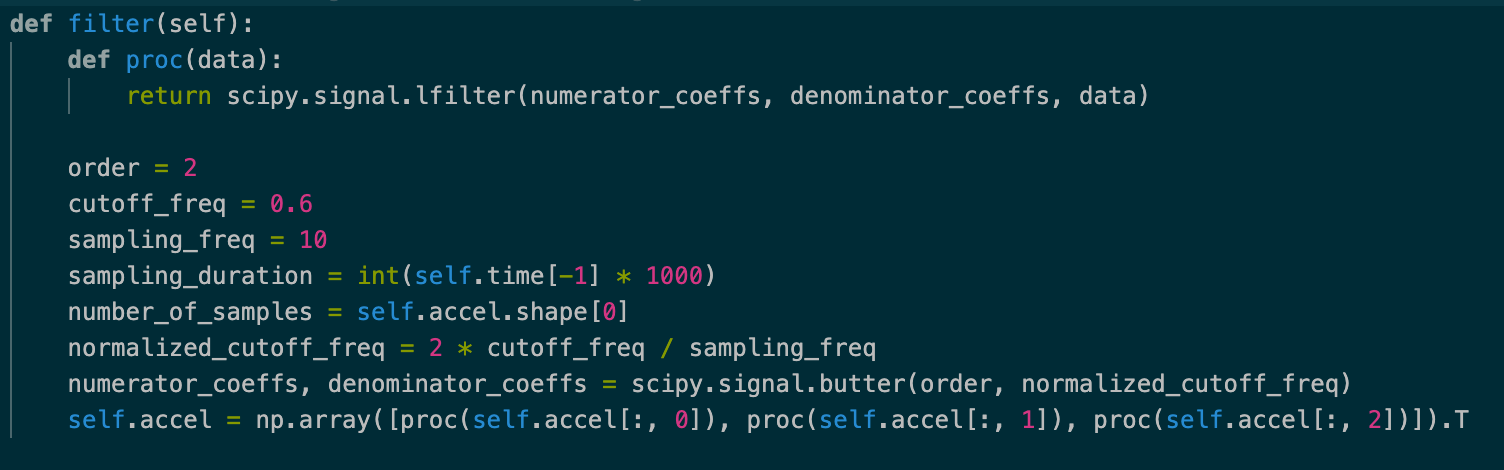
\includegraphics[width=0.7\textwidth]{images/filter.png}
    \end{center}
    \caption{метод GestrureData::filter}
\end{figure}
\begin{figure}[H]
  \begin{center}
      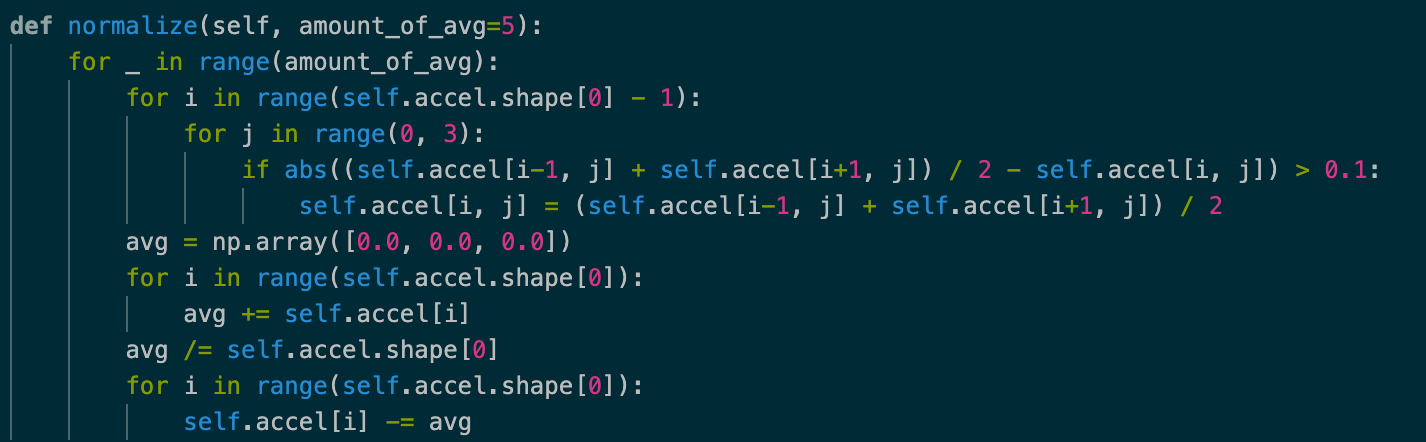
\includegraphics[width=0.7\textwidth]{images/normalize.png}
  \end{center}
  \caption{метод GestrureData::normalize}
\end{figure}
  \item после этого, показания акселерометра компенсируются, основываясь на данных гироскопа, для этого был реализован метод GestureData::normalize\_gyro,
  \begin{figure}[H]
    \begin{center}
        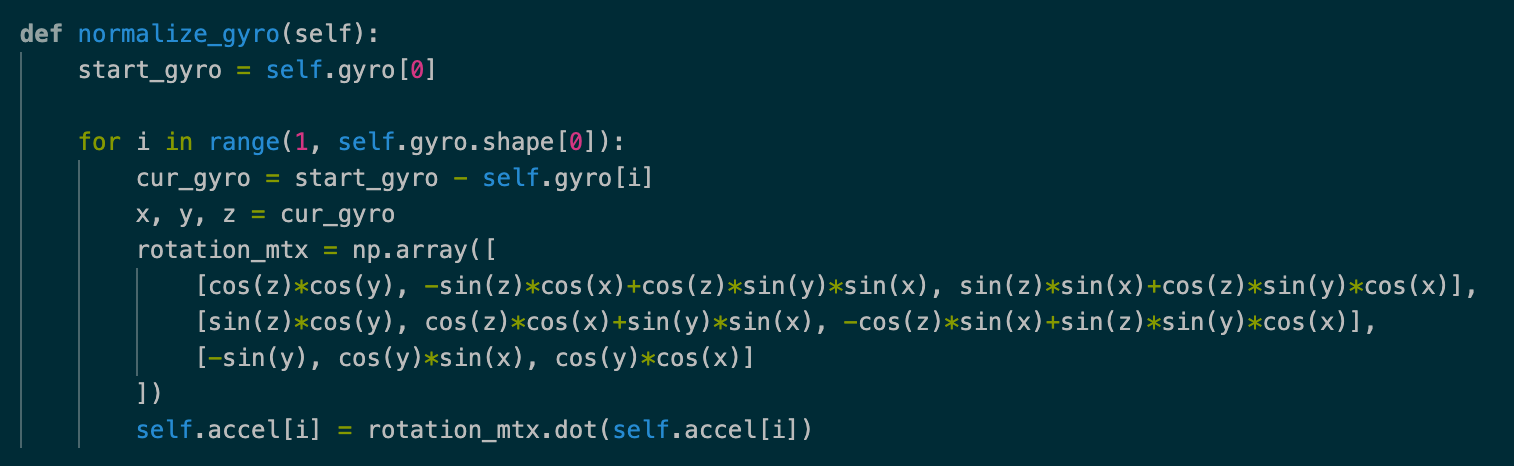
\includegraphics[width=0.7\textwidth]{images/norm_gyro.png}
    \end{center}
    \caption{метод GestrureData::normalize\_gyro}
  \end{figure}
  \item затем, выделяются такты и ищется усредненное движение, для этого был реализован метод GestureData ::find\_average,
  \item далее, полагая, что движение совершается в какой-то двумерной плоскости, находится наилучшая плоскость, внутри которой которой уже происходит поиск и классификация движения, для этого был реализован метод GestrureData::find\_pos, который находит движение и его проекции.
  \begin{figure}[H]
    \begin{center}
        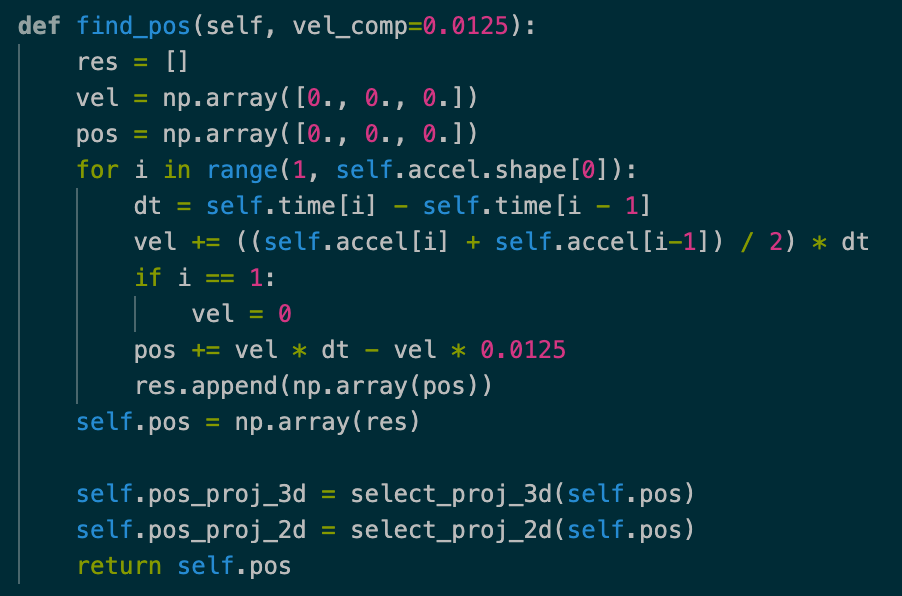
\includegraphics[width=0.7\textwidth]{images/find_pos.png}
    \end{center}
    \caption{метод GestrureData::find\_pos}
  \end{figure}
\end{itemize}

Так же были добавлены методы
\begin{itemize}
  \item GestureData::draw\_pos, который рисует графки движение в пространстве,
  \begin{figure}[H]
    \begin{center}
        \begin{tabular}{ccc}
            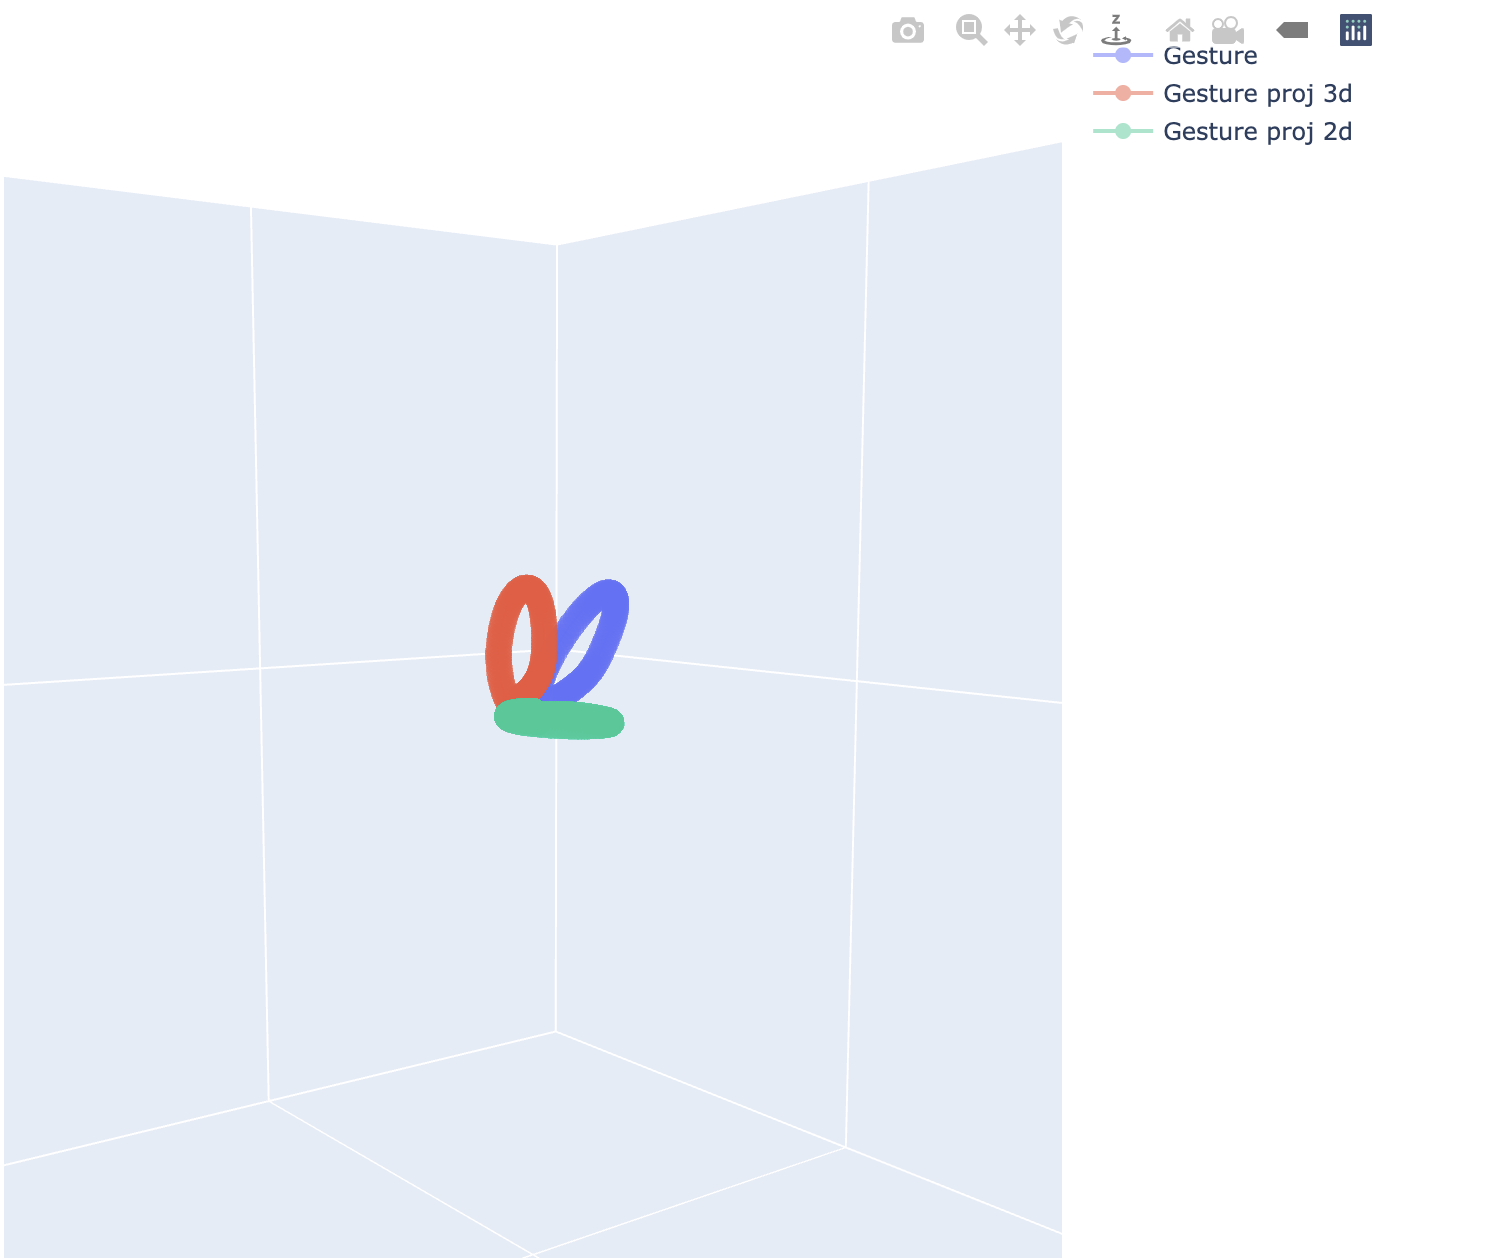
\includegraphics[width=0.45\textwidth]{images/draw_pos_1.png} & 
            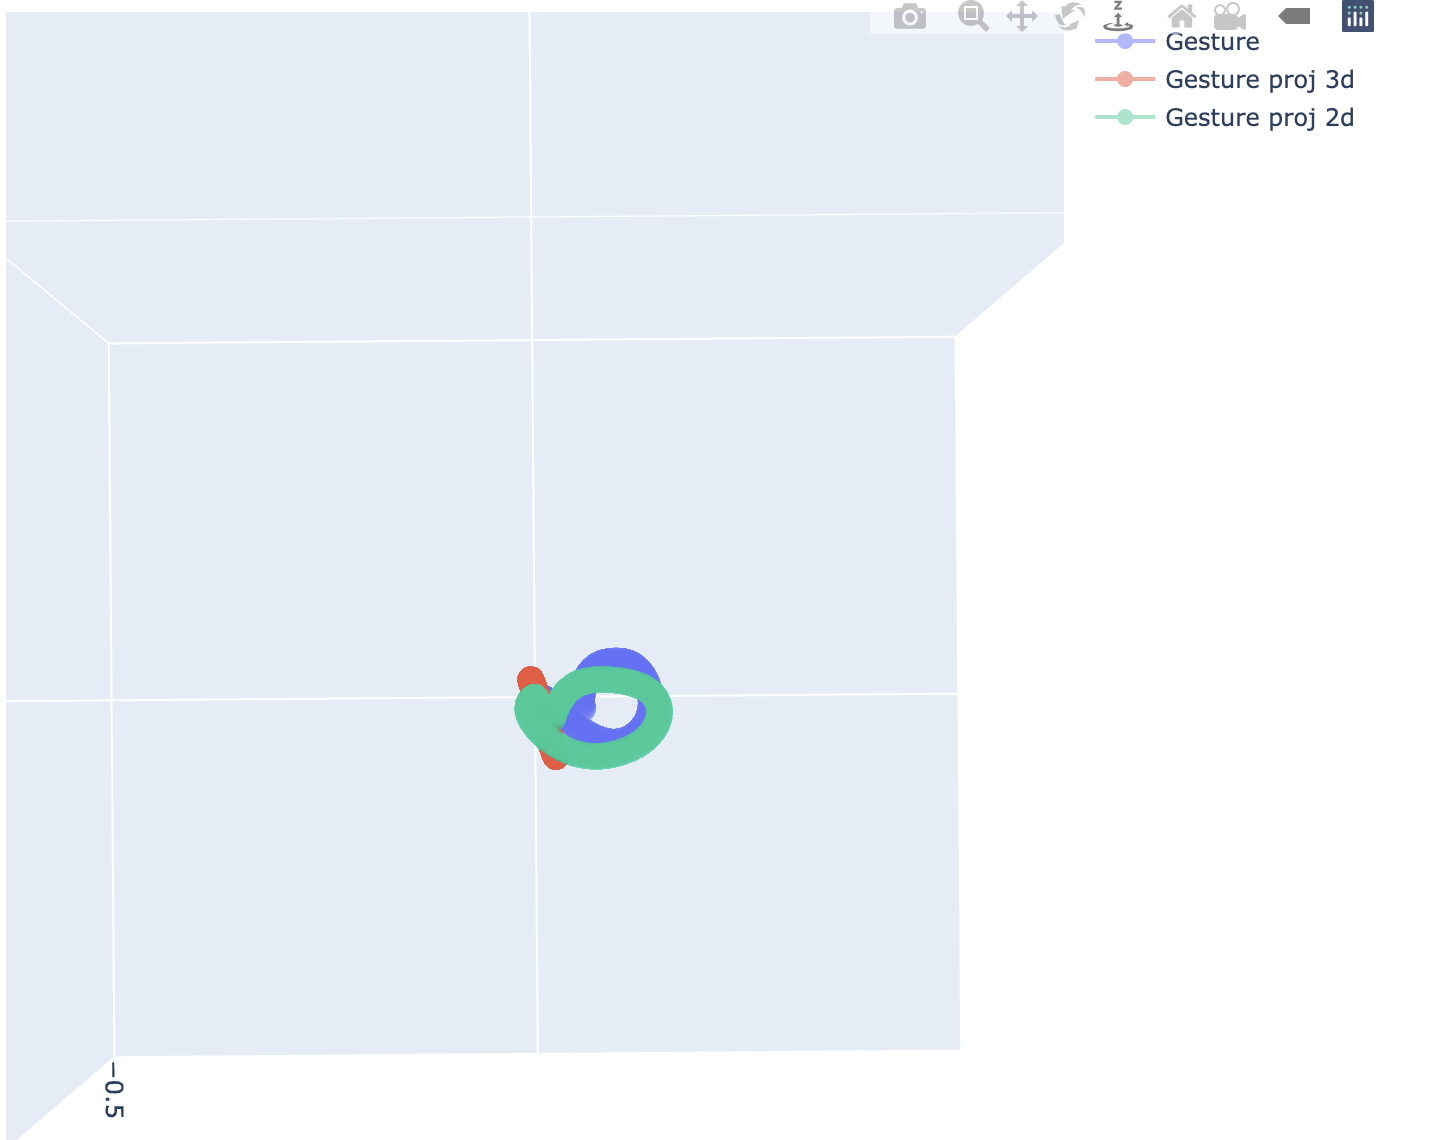
\includegraphics[width=0.45\textwidth]{images/draw_pos_2.png} \\
        \end{tabular}
    \end{center}
    \caption{Пример графика распознанного движения}
\end{figure}
  \item GestureData::pos\_to\_image, который создает картинку движения (используется при обучении и для визуализации в мобильном приложении)
  \begin{figure}[H]
    \begin{center}
        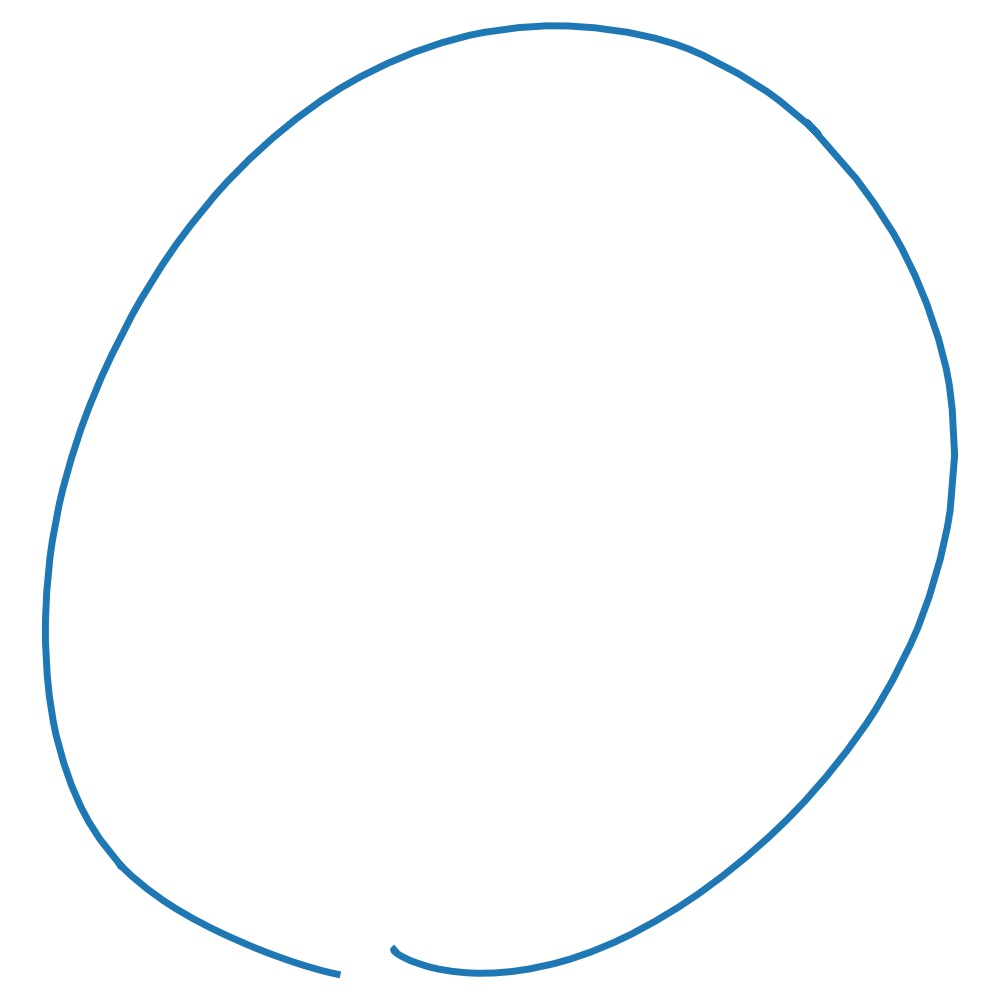
\includegraphics[width=0.4\textwidth]{images/pos_to_img_1.png}
    \end{center}
    \caption{Картинка, созданная методом GestureData::pos\_to\_image}
  \end{figure}
\end{itemize}

Для классификация движений был реализован класс Classifier, у которого определены следующее методы:
\begin{itemize}
  \item train(data). Данный метод используется для обучения модели.
  \item predict(data). Данный метод используется для предсказания движения.
  \item retrain. Данный метод используется для переобучения модели.
\end{itemize}

На сервере предусмотрены следующее обработчики запросов:
\begin{itemize}
  \item (POST) /train (name: String, gesture: GestrureData). При получении данного запроса происходит обучение модели на основе полученного усредненного движения в плоскости, полагая, что данное движение соответсвует классу name и при успешном обучении возвращается сообщение о успехе.
  \item (POST) /retrain. При получении данного запроса происходит переобучение модели.

  \item (POST) /predict (gesture: GestureData). При получении данного запроса происходит классификация движения на основе существующей модели и возвращается Gesture, в котором содержится класс, к которому относится данный жест, картинка с движением и данные о движение в плоскости и пространстве.
\end{itemize}



\subsubsection{Ссылка на библиотеку}
https://github.com/kaikash/hse-study-project/new\_lib